\section{Resultados}

\noindent A linha em vermelho indica a relação da quantidade de pessoas que 
aprovaram determinada expressura da massa.  A linha em azul mostra a relação da 
quantidade de pessoas que aprovaram a quantidade de ingredientes adicionados 
sobre da massa.  90\% prefere massas de 1,4 -- 2 centímetros, com recheio de 
1,8 -- 2,5 centímetros.  Em geral
a massa sempre mais fina que a quantidade de recheio, porém nenhuma aquém
da outra.

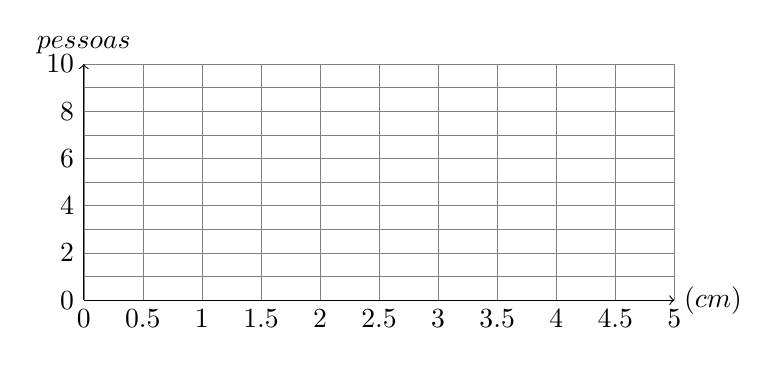
\begin{tikzpicture}[x=1.5cm,y=0.3cm]

  \def\xmin{0}
  \def\xmax{5}
  \def\ymin{0}
  \def\ymax{10}

  % grid
  \draw[style=help lines, ystep=1, xstep=0.5] (\xmin,\ymin) grid
  (\xmax,\ymax);

  % axes
  \draw[->] (\xmin,\ymin) -- (\xmax,\ymin) node[right] {$(cm)$};
  \draw[->] (\xmin,\ymin) -- (\xmin,\ymax) node[above] {$pessoas$};

  % xticks and yticks
  \foreach \x in {0,0.5,...,5}
    \node at (\x, \ymin) [below] {\x};
  \foreach \y in {0,2,...,10}
    \node at (\xmin,\y) [left] {\y};

  % generate and plot another a curve y = 0.1 x^2 + 2.5
  % this generates the files figure.parabola.gnuplot and figure.parabola.table 
  \draw[color=red, domain=\xmin:\xmax] plot[samples=100]
  function{10 * 2.7182818284 **(-1.8 * ((x-1.7)**2 / (1.1) ))} node [right] {};

  \draw[color=blue, domain=\xmin:\xmax] plot[samples=100]
  function{10 * 2.7182818284 **(-1.8 * ((x-2.1)**2 / (1.1) ))} node [right] {};
\end{tikzpicture}

%%%%%%%%%%%%%%%%%%%%%%%%%%%%%%%%%%%%%%%%%%%%%%%%%%%%%%%%%%%%%%%%%%%%%%%%%%%%%%%%


